\documentclass[hide notes,intlimits]{beamer}

\mode<presentation>
{
  \usetheme[footline]{PISMshade}
  \setbeamercovered{transparent}
}

%\documentclass{beamer}
%\documentclass[handout]{beamer}

%\mode<presentation>
%{
  %\usetheme{CambridgeUS}
  %\usetheme{Frankfurt}
  %\usetheme{Singapore}
  %\usecolortheme{crane}
  %\usefonttheme{professionalfonts}
  %\usefonttheme[onlymath]{serif}
  
  %\setbeamertemplate{blocks}[rounded][shadow=true]
%}

\usepackage{pgfpages}

\usepackage{alltt,verbatim,amsmath,times,empheq}
\usepackage{bm}
\usepackage[english]{babel}
\usepackage[utf8]{inputenc}

\usepackage{tikz}

%\usepackage{times}
%\usepackage[T1]{fontenc}
% Or whatever. Note that the encoding and the font should match. If T1
% does not look nice, try deleting the line with the fontenc.

%\usepackage{hyperref}

%\usepackage{pdfanim}
%\usepackage{multimedia,xmpmulti}

%\PDFAnimLoad[width=\textwidth,loop,interval=40]{exp3a}{exp3a/pic}{310}%

\usepackage{animate}

\definecolor{dark red}{HTML}{E41A1C}
\definecolor{dark green}{HTML}{4DAF4A}
\definecolor{dark violet}{HTML}{984EA3}
\definecolor{dark blue}{HTML}{084594}
\definecolor{dark orange}{HTML}{FF7F00}
\definecolor{light blue}{HTML}{377EB8}
\definecolor{light red}{HTML}{FB9A99}
\definecolor{light violet}{HTML}{CAB2D6}

\setbeamercolor{boxed}{fg=black,bg=uaf yellow}

\newcommand{\CC}{\mathbb{C}}
\newcommand{\NN}{\mathbb{N}}
\newcommand{\RR}{\mathbb{R}}
\newcommand{\ZZ}{\mathbb{Z}}
\newcommand{\Acal}{\mathcal{A}}
\newcommand{\Bcal}{\mathcal{B}}
\newcommand{\Ccal}{\mathcal{C}}
\newcommand{\Ncal}{\mathcal{N}}
\newcommand{\Kcal}{\mathcal{K}}

\newcommand{\bF}{\mathbf{F}}
\newcommand{\bQ}{\mathbf{Q}}
\newcommand{\bU}{\mathbf{U}}
\newcommand{\bbU}{\bar{\bU}}
\newcommand{\bu}{\mathbf{u}}
\newcommand{\bv}{\mathbf{v}}
\newcommand{\bx}{\mathbf{x}}

\newcommand{\Div}{\nabla\cdot}
\newcommand{\eps}{\epsilon}
\newcommand{\grad}{\nabla}
\newcommand{\lap}{\triangle}
\DeclareMathOperator{\trace}{tr}
\renewcommand{\bar}{\overline}

\newcommand{\ddx}[1]{\frac{\partial #1}{\partial x}}
\newcommand{\ddy}[1]{\frac{\partial #1}{\partial y}}
\newcommand{\pp}[2]{\frac{\partial #1}{\partial #2}}
\newcommand{\ppt}[1]{\frac{\partial #1}{\partial t}}
\newcommand{\ppT}[1]{\frac{\partial #1}{\partial T}}
\newcommand{\ppx}[1]{\frac{\partial #1}{\partial x}}
\newcommand{\ppy}[1]{\frac{\partial #1}{\partial y}}
\newcommand{\ppz}[1]{\frac{\partial #1}{\partial z}}
\newcommand{\ppxx}[1]{\frac{\partial^2 #1}{\partial x^2}}
\newcommand{\ppzz}[1]{\frac{\partial^2 #1}{\partial z^2}}

\newcommand{\Tnorm}[1]{\left|\!\left|\!\left|#1\right|\!\right|\!\right|}
\newcommand{\rhow}{\rho_{\text{w}}}
\newcommand{\Wq}{W^{1,q}(\Omega)}
\newcommand{\half}{\frac12}

%\setbeamercolor{redtext}{fg=red!80!black}
\setbeamercolor{redtext}{fg=red!94!black}
%\setbeamercolor{greentext}{fg=green!80!black}
\setbeamercolor{greentext}{fg=green!60!black}
%\setbeamercolor{bluetext}{fg=blue!70!black}
\setbeamercolor{bluetext}{fg=blue!90!black}
\setbeamercolor{yellowtext}{fg=yellow!95!black}
\setbeamercolor{orangetext}{fg=yellow!50!red}

\newcommand{\green}{\usebeamercolor[fg]{greentext}}
\newcommand{\blue}{\usebeamercolor[fg]{bluetext}}
\newcommand{\red}{\usebeamercolor[fg]{redtext}}

\renewcommand{\L}{\emph{Left}}
\newcommand{\R}{\emph{Right}}

\newcommand{\contactslipslide}{
\begin{frame}{sheets versus streams versus shelves}

\begin{columns}
\begin{column}{0.35\textwidth}
\small
\begin{itemize}
\small
\item non-sliding portions of ice sheets flow by shear deformation
\item ice streams slide: \alert{contact slip}
\item ``ice shelves'' are floating thick ice
\item ice shelves flow by extension
  \begin{itemize}
  \scriptsize
  \item[$\circ$] ``membrane'' or ``plug'' flow
  \end{itemize}
\end{itemize}
\end{column}

\begin{column}{0.65\textwidth}
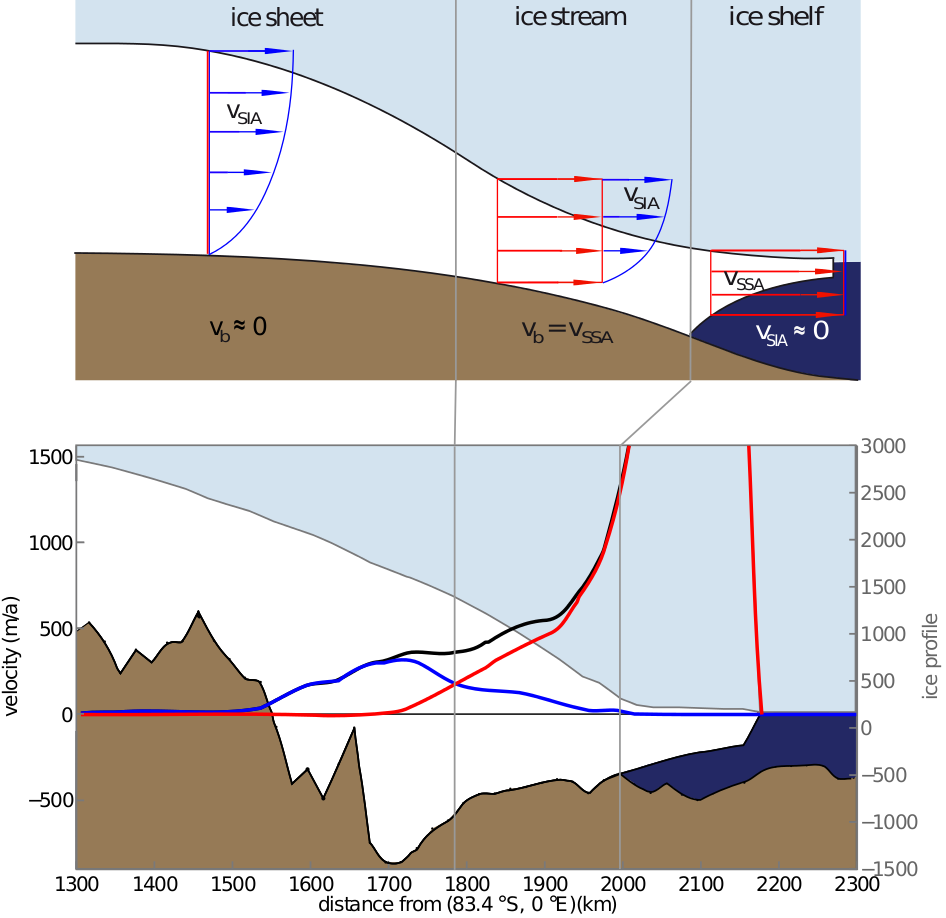
\includegraphics[width=1.1\textwidth]{siassacartoon-lambert}

\begin{center}
\vspace{-0.18in}
\tiny [Lambert glacier and Amery ice shelf, Antarctic]
\end{center}
\end{column}
\end{columns}
\end{frame}
}




\title{Flowing ice in glaciers and ice sheets \\ (as applied math)}

\author[Bueler]{Ed Bueler}

\institute[UAF]{
  \tiny Dept of Mathematics and Statistics \\

  University of Alaska Fairbanks
}

\date{\tiny 18 May, 2018}


\setbeamerfont{date}{size=\scriptsize}

\subject{ice sheets, glaciers, numerical analysis, applied mathematics}


%\begin{comment}
\AtBeginSection[]
{
  \begin{frame}<beamer>
    \frametitle{Outline}
    \tableofcontents[currentsection,hideallsubsections]
  \end{frame}
}
%\end{comment}


\begin{document}
\graphicspath{{../../old/commonfigs/}{../../figures/}}

\begin{frame}
  \titlepage
  \begin{center}
  \tiny supported by NASA grants NNX13AM16G, NNX16AQ40G, NNX17AG65G 
  \end{center}
\end{frame}



% NO OUTLINE BECAUSE ONE APPEARS AT START OF EACH SECTION ?
%\begin{comment}
%\begin{frame}
  %\frametitle{Outline}
  %\tableofcontents[hideallsubsections]
  % You might wish to add the option [pausesections]
%\end{frame}
%\end{comment}


\section[the alien view]{the alien physicist view of Greenland}

\setbeamertemplate{background canvas}{
     \tikz{\node[inner sep=0pt,opacity=1] {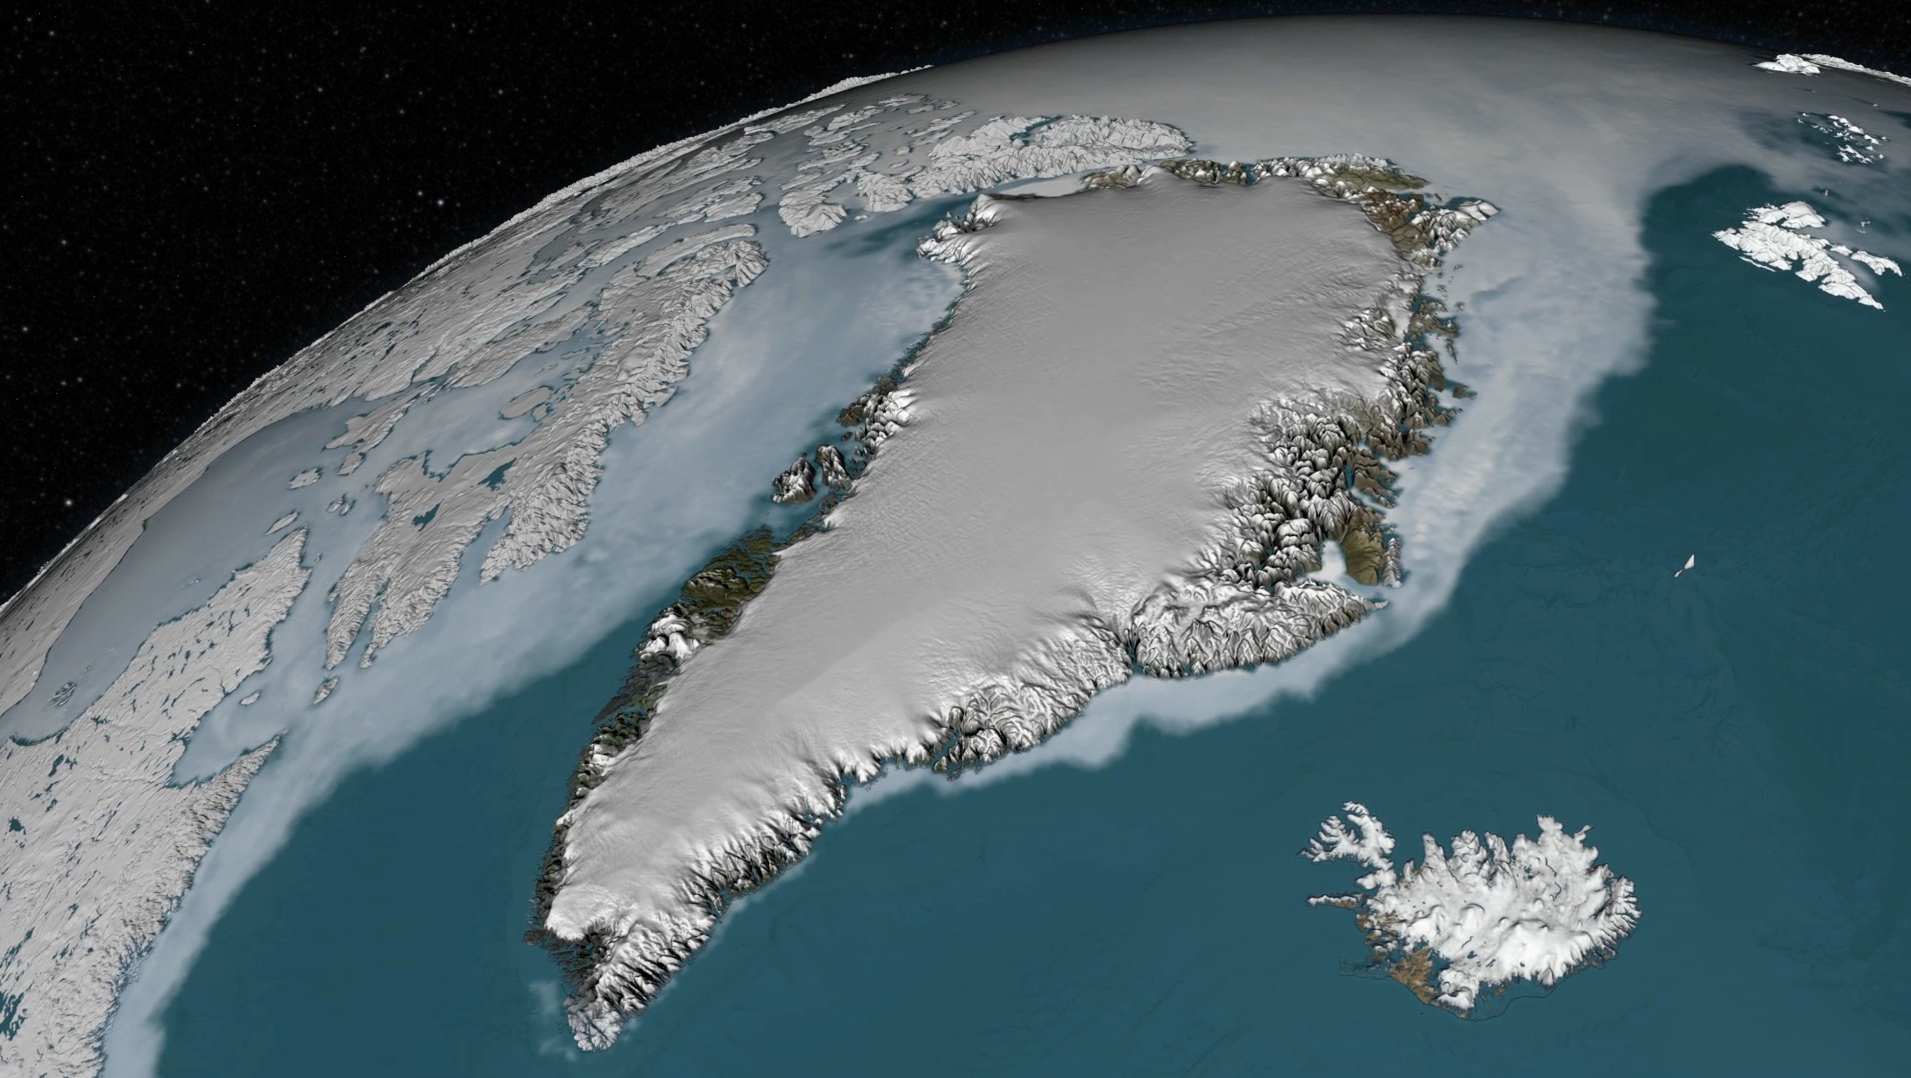
\includegraphics[height=\paperheight,width=\paperwidth]{nasa-mapping-greenland-ice-sheet}};}
} 

% show:
% (1) GRACE movie
% (2) Andy PISM: observed versus modeled surface velocity

\begin{frame}{}

\only<2>{
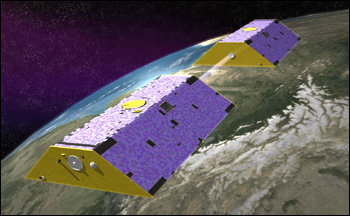
\includegraphics[width=0.3\textwidth]{grace-satellites}

\vfill \hfill 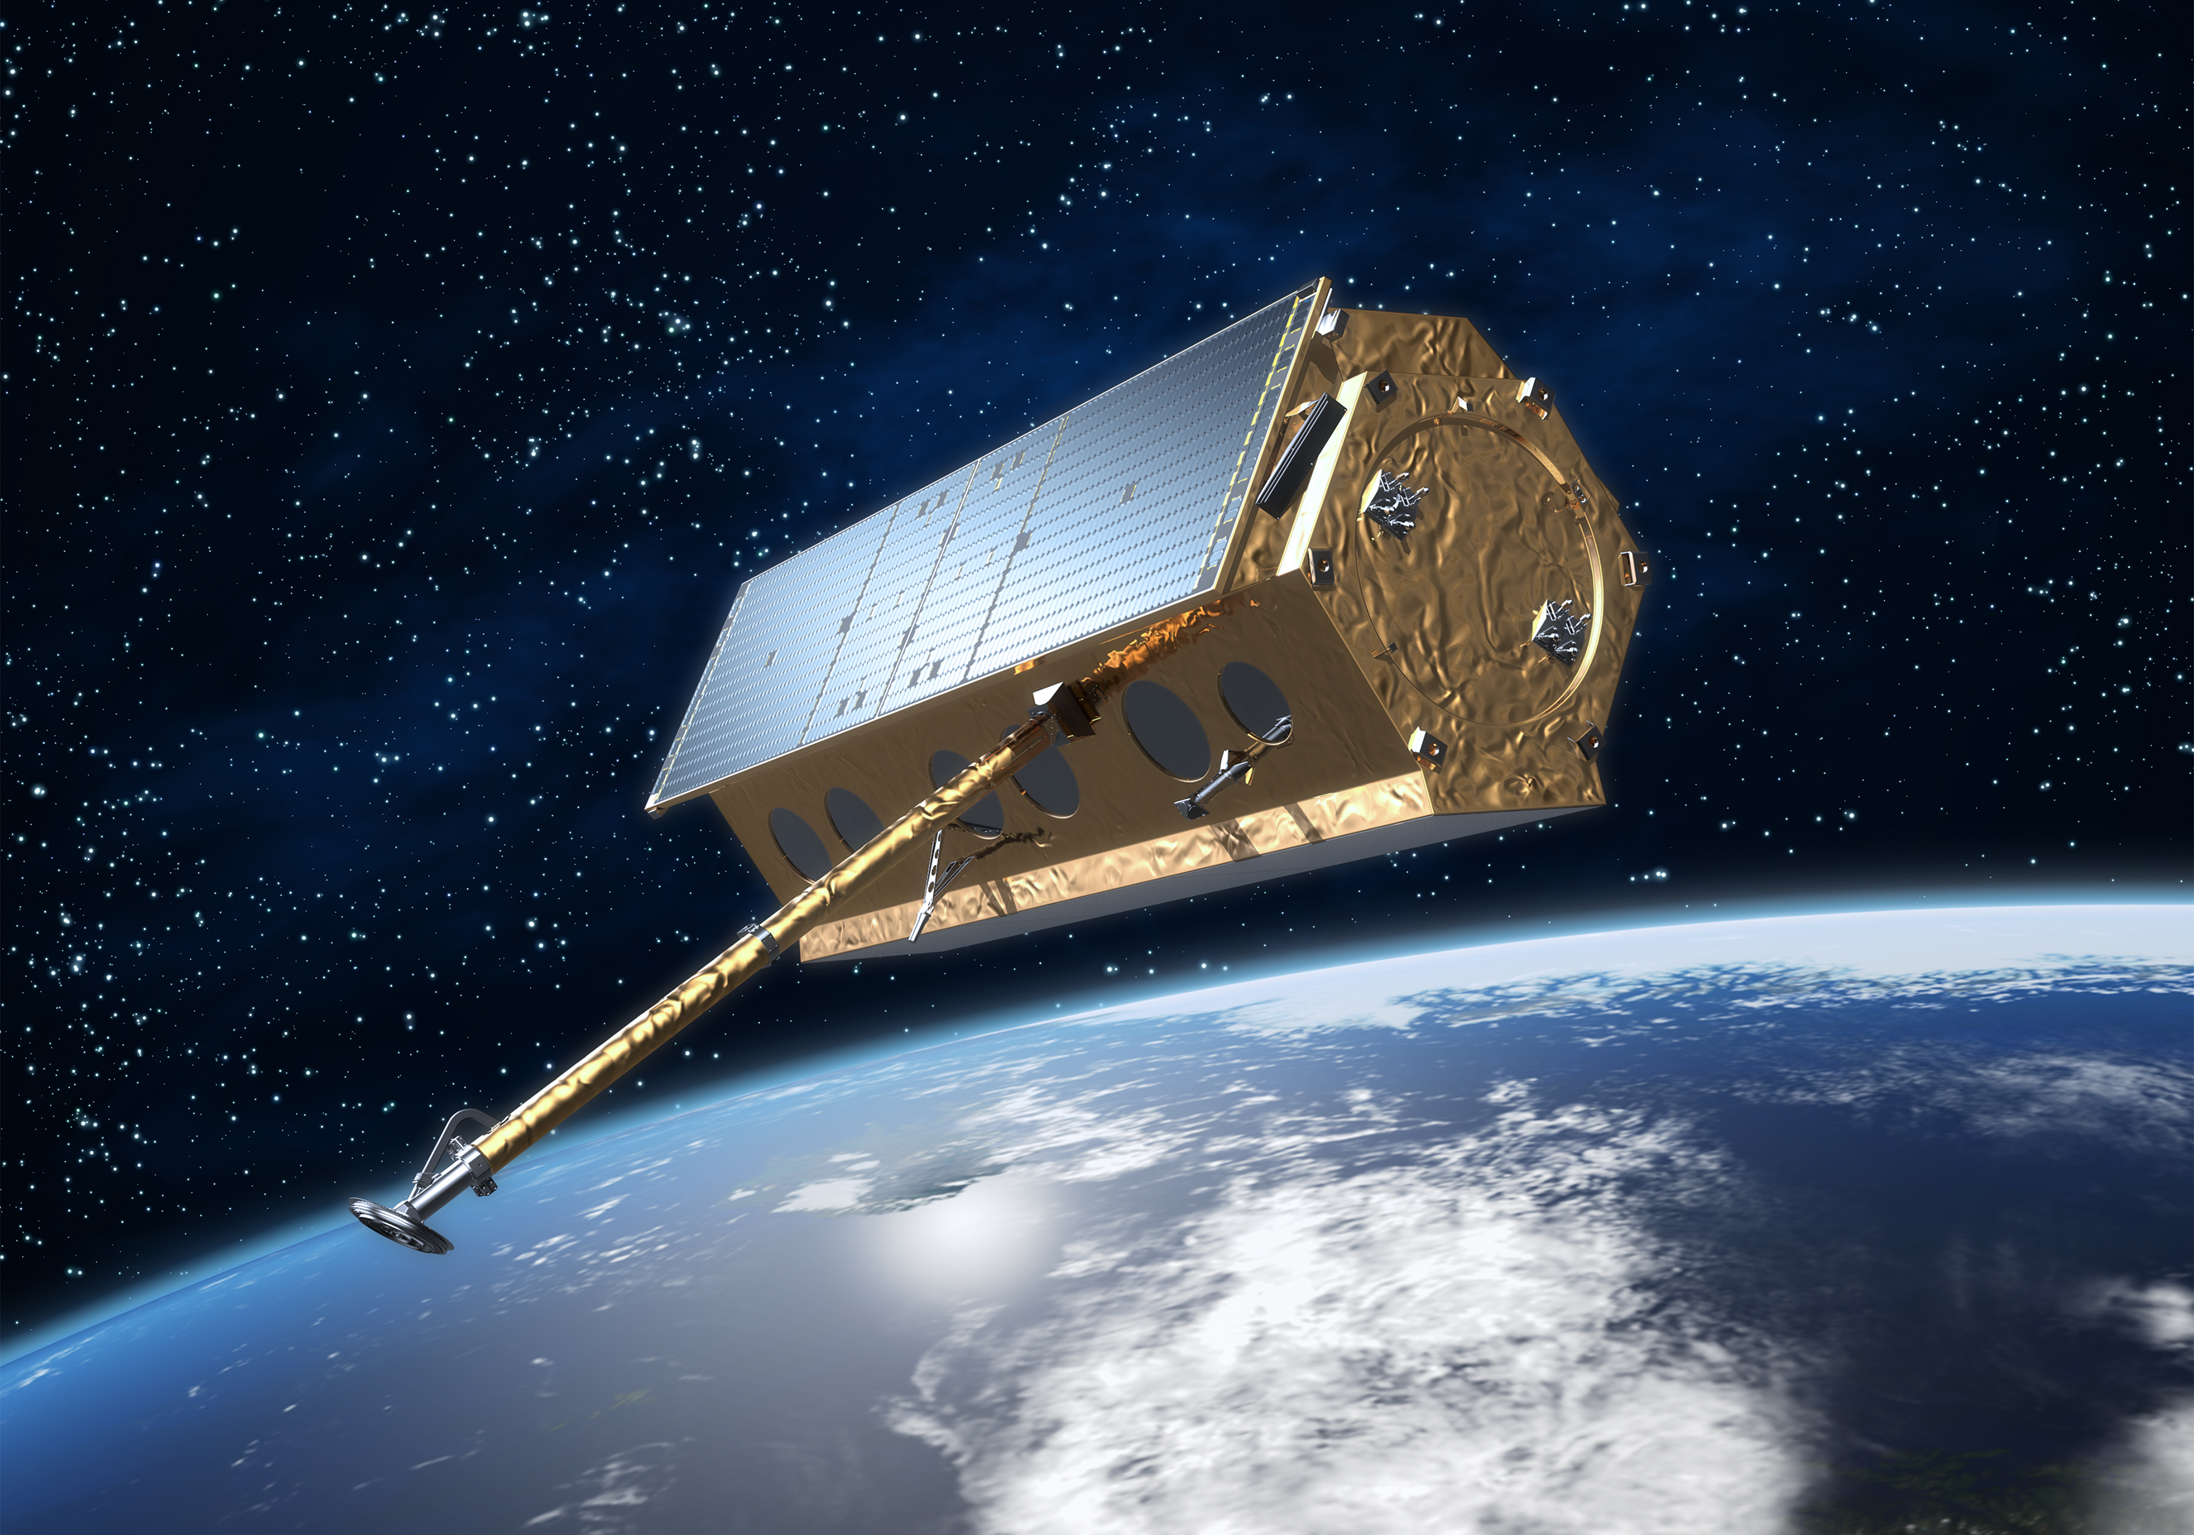
\includegraphics[width=0.3\textwidth]{TerraSAR_n}
}
\end{frame}

\setbeamertemplate{background canvas}{}


\begin{frame}{FIXME movies from GRACE and andy/PISM}
\end{frame}


\section[intro to ice flow]{an introduction to flowing ice}


\begin{frame}{ice in glaciers is a viscous fluid}
\begin{columns}
\begin{column}{0.65\textwidth}
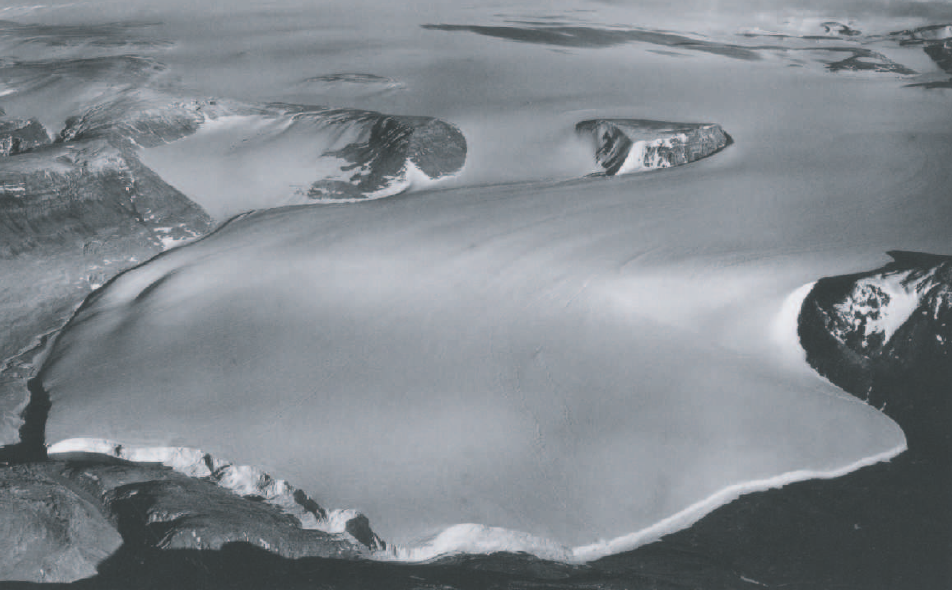
\includegraphics[width=1.0\textwidth]{polaris}
\end{column}
\begin{column}{0.35\textwidth}
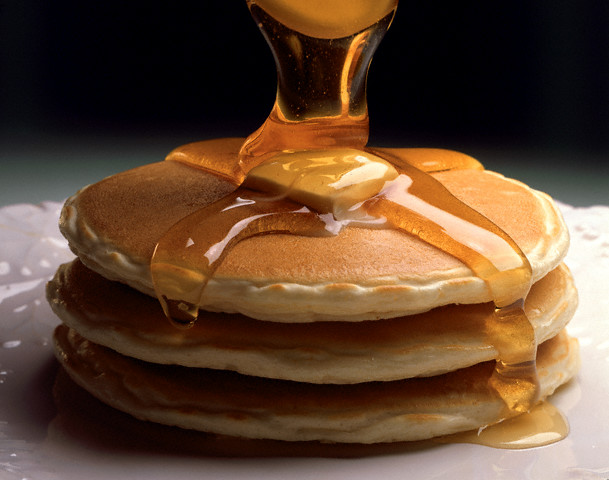
\includegraphics[width=1.0\textwidth]{pancakes}
\end{column}
\end{columns}

\bigskip
\begin{itemize}
\item glaciers and ice sheets are viscous flows at the large scale
  \begin{itemize}
  \item[$\circ$] at a smaller scale they are ice crystals
  \item[$\circ$] at yet-smaller scale they are molecules \dots atoms \dots quarks
  \end{itemize}
\item \emph{usage}: ``ice sheets'' are big, shallow glaciers
\end{itemize}
\end{frame}


\begin{frame}{ice sheets are shallow}

\begin{itemize}
\item cross section of Greenland ice sheet at $71^\circ$ N
  \begin{itemize}
  \item[$\circ$] {\color{dark green}{green}} and {\color{dark blue}{blue}}: vertically-exaggerated version
  \item[$\circ$] in {\color{dark red}{red}}: without vertical exaggeration
  \end{itemize}
\end{itemize}
\normalsize

  \begin{center}
    \tikz{\draw[<->] (0.0,-2.9) -- node [midway, left] {3500 m} (0.0,2.7);}  \quad 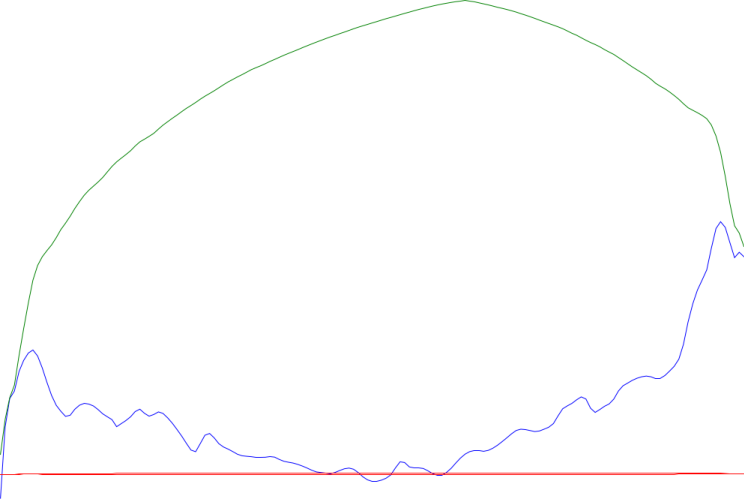
\includegraphics[width=0.7\textwidth]{greentransecttrimmed}
    
    \bigskip
    \qquad\qquad\qquad \tikz{\draw[<->] (-4.1,0.0) -- node [midway, below] {750 km} (4.1,0.0);}
  \end{center}
\end{frame}


\begin{frame}{what is a fluid?}

\bigskip
\begin{itemize}
\item seriously
\item<2-> is it just a collection of particles?
\item<3-> a fluid is a mathematical abstraction
  \begin{itemize}
  \item<3->[$\circ$]   a continuous function $y=f(x)$ is also an abstraction
  \end{itemize}
\item<4-> primary variables:
  \begin{itemize}
  \item<4->[$\circ$]   velocity $\mathbf{u}(\bx,t)$
  \item<4->[$\circ$]   pressure $p(\bx,t)$
  \item<4->[$\circ$]   density $p(\bx,t)$
  \end{itemize}
\end{itemize}
\end{frame}



\begin{frame}{ice in glaciers is a viscous fluid}

\begin{itemize}
\item these are fluids:
  \begin{itemize}
  \item[$\circ$] air
  \item[$\circ$] liquid water
  \item[$\circ$] syrup
  \item[$\circ$] glacier ice
  \end{itemize}
\item they are are all modeled as \alert{incompressible viscous fluids}
\item if a glacier was a ``typical'' incompressible viscous fluid we would describe it with Navier-Stokes equations:
\begin{align*}
\nabla \cdot \mathbf{u} &= 0 &&\qquad \text{\emph{incompressibility}} \\
\rho \left(\mathbf{u}_t + \mathbf{u}\cdot\nabla \mathbf{u}\right) &= -\nabla p + \nu \nabla^2 \mathbf{u} + \rho \mathbf{g} &&\qquad \text{\emph{stress balance}}
\end{align*}
\item in 3D these equations are known to be hard
  \begin{itemize}
  \item[$\circ$] \$1 million Clay Institute prize \dots unclaimed for 18 years \dots for proving there are solutions
  \end{itemize}
\end{itemize}
\end{frame}



\begin{frame}{ice is a weird viscous fluid}

\begin{itemize}
\item \dots but glacier ice is not a typical fluid!
\item for example, these are not relevant in glacier flow but they are a big deal for weather and climate models of the atmosphere and ocean:
  \begin{itemize}
  \item[$\circ$] turbulence
  \item[$\circ$] convection
  \item[$\circ$] coriolis force
  \item[$\circ$] density variations
  \end{itemize}
\end{itemize}
\end{frame}


\begin{frame}{ice is a slow, shear-thinning viscous fluid}

\begin{itemize}
\item our glacier fluid is
  \begin{enumerate}
  \item ``slow'' is a technical term:\footnote{the Froude number is approximately $10^{-15}$}
    $$\rho \left(\mathbf{u}_t + \mathbf{u}\cdot\nabla \mathbf{u}\right) \approx 0 \qquad \iff \qquad \begin{pmatrix} \text{forces of inertia} \\ \text{are negligible} \end{pmatrix}$$
  \item non-Newtonian (shear-thinning):
    $$\text{viscosity $\nu$ is not constant}$$
  \end{enumerate}

\medskip
\item for ``shear-thinning'' there is a power law (``Glen law''):
  $$(\text{strain rate}) = A (\text{shear stress})^n$$
where $A>0$ is the ice ``softness''
\item $1.8 < n < 4.0$ ?  \quad when in doubt: \alert{$n=3$}
\end{itemize}
\end{frame}


\begin{frame}{ice is a slow, shear-thinning viscous fluid}

\begin{itemize}
\item notation:
  \begin{itemize}
  \item[$\circ$] $\tau_{ij}$ is deviatoric stress tensor
  \item[$\circ$] $\mathbf{D}u_{ij}$ is strain rate tensor
  \end{itemize}
\smallskip
\item the standard ice flow model is Glen-law Stokes:
\begin{align*}
\nabla \cdot \mathbf{u} &= 0 &&\text{\emph{incompressibility}} \\
0 &= - \nabla p + \nabla \cdot \tau_{ij} + \rho \mathbf{g} &&\text{\emph{slow stress balance}} \\
\mathbf{D}u_{ij} &= A \left|\tau_{ij}\right|^2 \tau_{ij} &&\text{\emph{Glen flow law}}
\end{align*}
\end{itemize}
\end{frame}


\section[big questions]{big picture questions for ice flow models}


\contactslipslide


\begin{frame}{outstanding viscous flows}

\begin{itemize}
\item ice sheets have four outstanding properties \emph{as viscous flows}:
  \begin{enumerate}
  \item \alert{slow}
  \item \alert{shear-thinning}
  \item \alert{shallow}
  \item \alert{contact slip}
  \end{enumerate}
\end{itemize}
\end{frame}


\begin{frame}
  \frametitle{big picture: ice sheet flow interacts with climate}

\medskip
\small
\begin{itemize}
\item \emph{mass and energy inputs}: (1) snow adds, (2) sun heats, (3) ocean heats, (4) earth heats
\item \emph{mass outputs}: (1) surface meltwater, (2) basal meltwater, (3) ice discharge
\end{itemize}

\begin{center}
  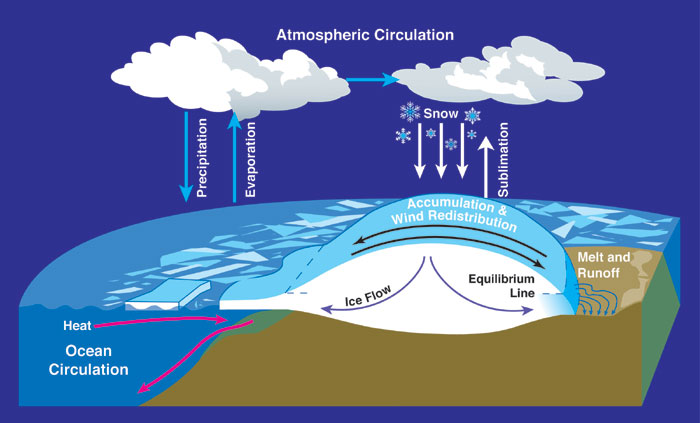
\includegraphics[width=0.75\textwidth]{mass-bal-atmos}
\end{center}
\end{frame}


\begin{frame}
  \frametitle{big picture: ice sheets are meltable ice sitting above sea level}

\small
\begin{itemize}
\item Greenland ice sheet mass is $2.7 \times 10^9$ Gt \quad $(\approx \text{km}^3)$ % = 2.93466 10^6 km^3  volume, from SeaRISE-Greenland 5km data
\item if \emph{all} Greenland ice melts: 7 m of sea level rise
\item if \emph{all} Antarctic ice melts: 61 m of sea level rise
\end{itemize}
\end{frame}



\section[numerical models]{numerical models of ice sheets}


\begin{frame}
  \frametitle{the main variables}

\begin{center}
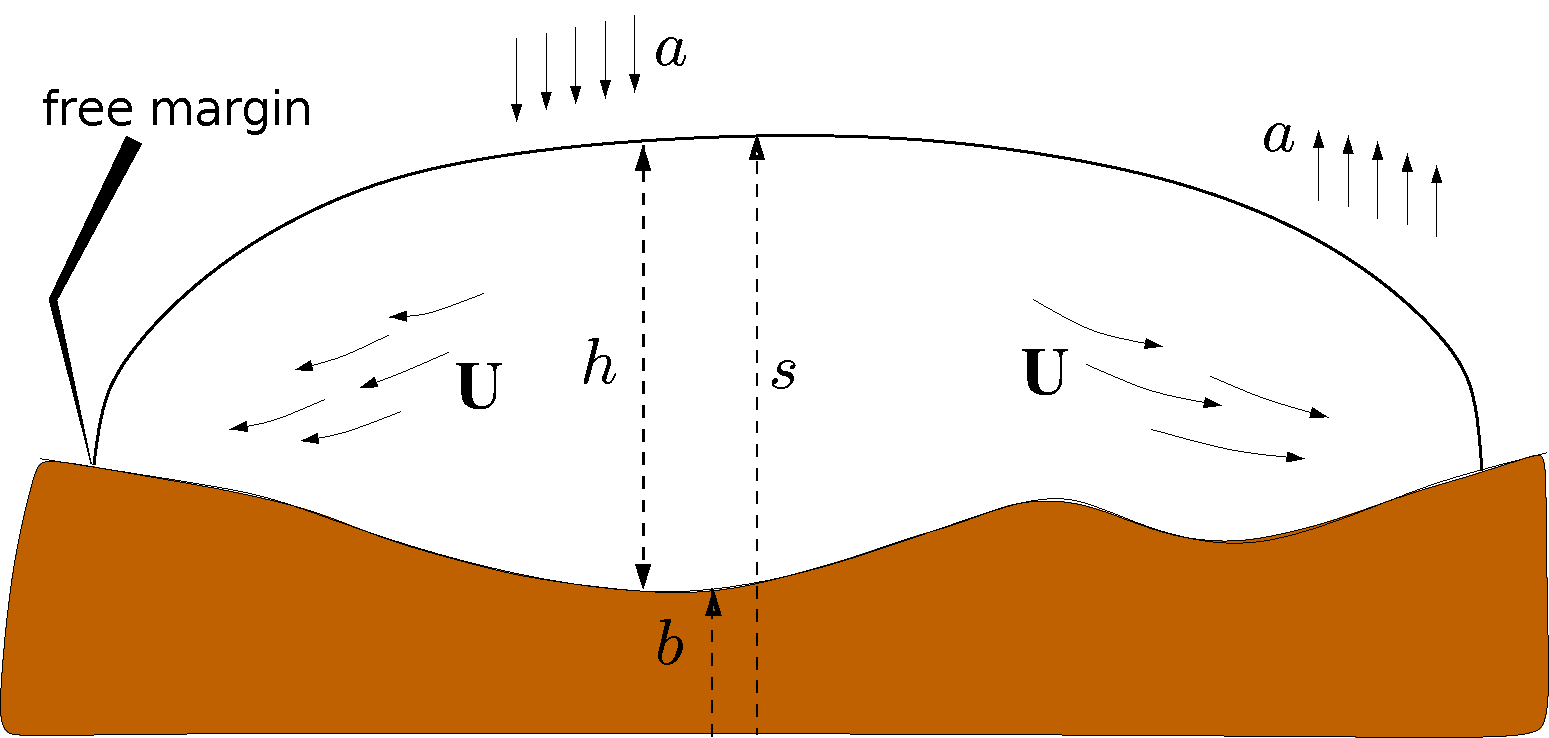
\includegraphics[width=0.7\textwidth]{groundedscheme}
\end{center}

\begin{itemize}
\small
\item $s=$ ice surface elevation
\item $b=$ bedrock elevation
\item $h=$ ice thickness $ = s-b$
\item ${\bf U}=$ horizontal velocity field
\item $a=$ surface mass balance (accumulation)
\end{itemize}

\begin{alertblock}{obvious idea: ice surface $s$ is always above the bedrock $b$}
\end{alertblock}
\end{frame}


\begin{frame}
  \frametitle{ice sheets: a mathematical modeling analogy}

\begin{columns}
\begin{column}{0.35\textwidth}
\begin{itemize}
\item ice sheet surface \\ = \alert{membrane}
\item bedrock = \alert{obstacle}
\end{itemize}
\vfill
\begin{center}
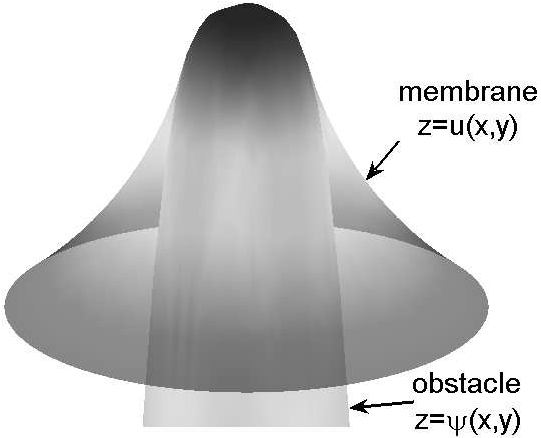
\includegraphics[width=1.1\textwidth]{classicalobs}
\end{center}
\end{column}
\begin{column}{0.65\textwidth}
\begin{center}
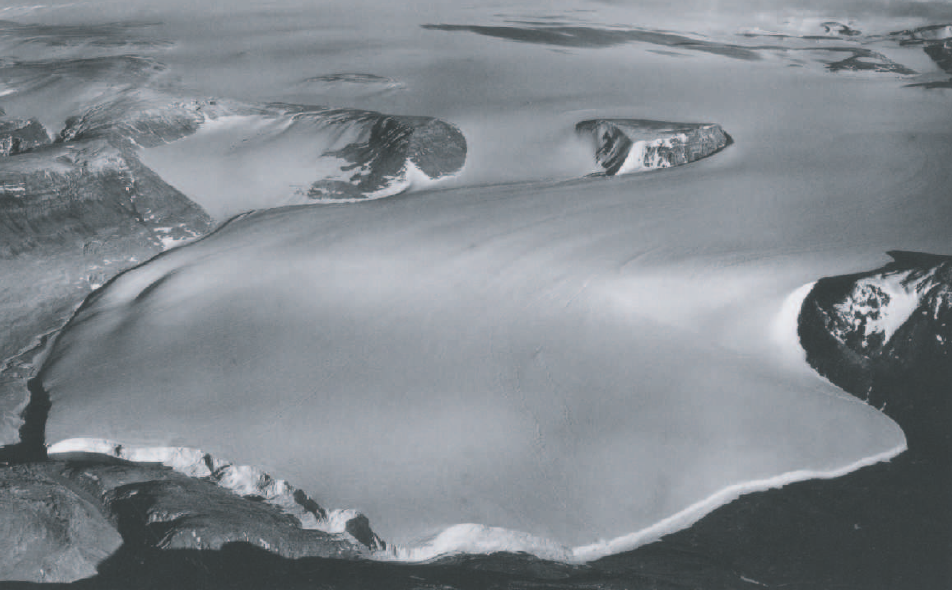
\includegraphics[width=0.8\textwidth]{polaris} \\
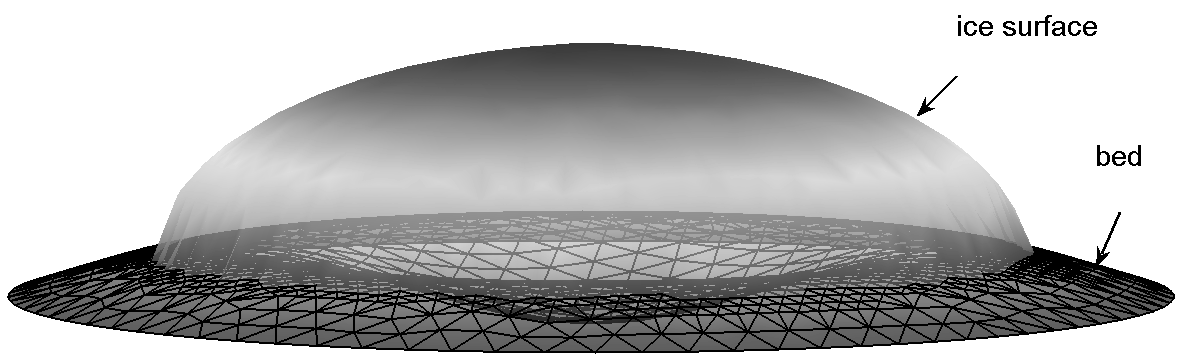
\includegraphics[width=\textwidth]{capnonflatobs}
\end{center}
\end{column}
\end{columns}
\end{frame}



\begin{frame}
  \frametitle{shallow ice approximation (SIA)}

\begin{itemize}
\item SIA = lubrication approximation of Glen-law Stokes model earlier
\item good approximation when:
  \begin{itemize}
  \item[$\circ$] sliding is small or zero
  \item[$\circ$] bedrock slope is modest
  \end{itemize}
\item derive SIA equations by scaling Stokes:
  \begin{itemize}
  \item[$\circ$] $[h]$ is a typical thickness scale
  \item[$\circ$] $[x]$ is a typical width scale
  \item[$\circ$] small parameter is $\eps = [h] / [x]$
  \end{itemize}
\end{itemize}
\end{frame}



\begin{frame}
  \frametitle{SIA: velocity}
 
\begin{itemize}
\item horizontal ice velocity is given by: 
  $${\bf U}  =  - \frac{2 A}{4} (\rho g)^{3} \left[ (s-b)^4 - (s - z)^4  \right] 
|\nabla s |^{2} \nabla s$$
\item no PDE needs to be solved to compute velocity!
\end{itemize}
\end{frame}



\begin{frame}
  \frametitle{SIA: steady state}

\begin{itemize}
\item mass conservation in steady state: 
  $$\Div \left(  \int_b^s {\bf U}\, dz \right)  =  a$$
\item shallow ice approximation + (steady) mass conservation:
  $$- \Div \left(\Gamma (s-b)^5 | \nabla s |^2 \nabla s  \right) =  a$$
  \begin{itemize}
  \vspace{-0.2in}
  \item[$\circ$] this is the major SIA equation (\dots a PDE?)
  \item[$\circ$] computes ice surface $s$
  \item[$\circ$] constant $\Gamma > 0$ combines $\rho,g,A$
  \item[$\circ$] coefficient $(s-b)^5 \to 0$ at margins
  \end{itemize}
\end{itemize}
\end{frame}


\begin{frame}{movie of time-dependent SIA}

\begin{columns}
\begin{column}{0.4\textwidth}
\small
\begin{itemize}
\item at right is the Halfar similarity solution
\item an exact, time-dependent, zero mass balance solution where the $t\to 0^+$ limit is a delta function
\item compare Barenblatt solution of porous medium equation
\end{itemize}
\end{column}

\begin{column}{0.65\textwidth}
\vspace{-0.25in}

\begin{center}
\animategraphics[autoplay,loop,height=4.7cm]{4}{../commonfigs/animhalfar/halfar}{0}{26}

\bigskip
\tiny
frames from $t=4$ months to $t = 10^6$ years,

equal spaced in \emph{exponential} time
\end{center}
\end{column}
\end{columns}
\end{frame}


\contactslipslide


\begin{frame}
  \frametitle{ice shelf versus sea ice}

\begin{center}
\vspace{-0.2in}

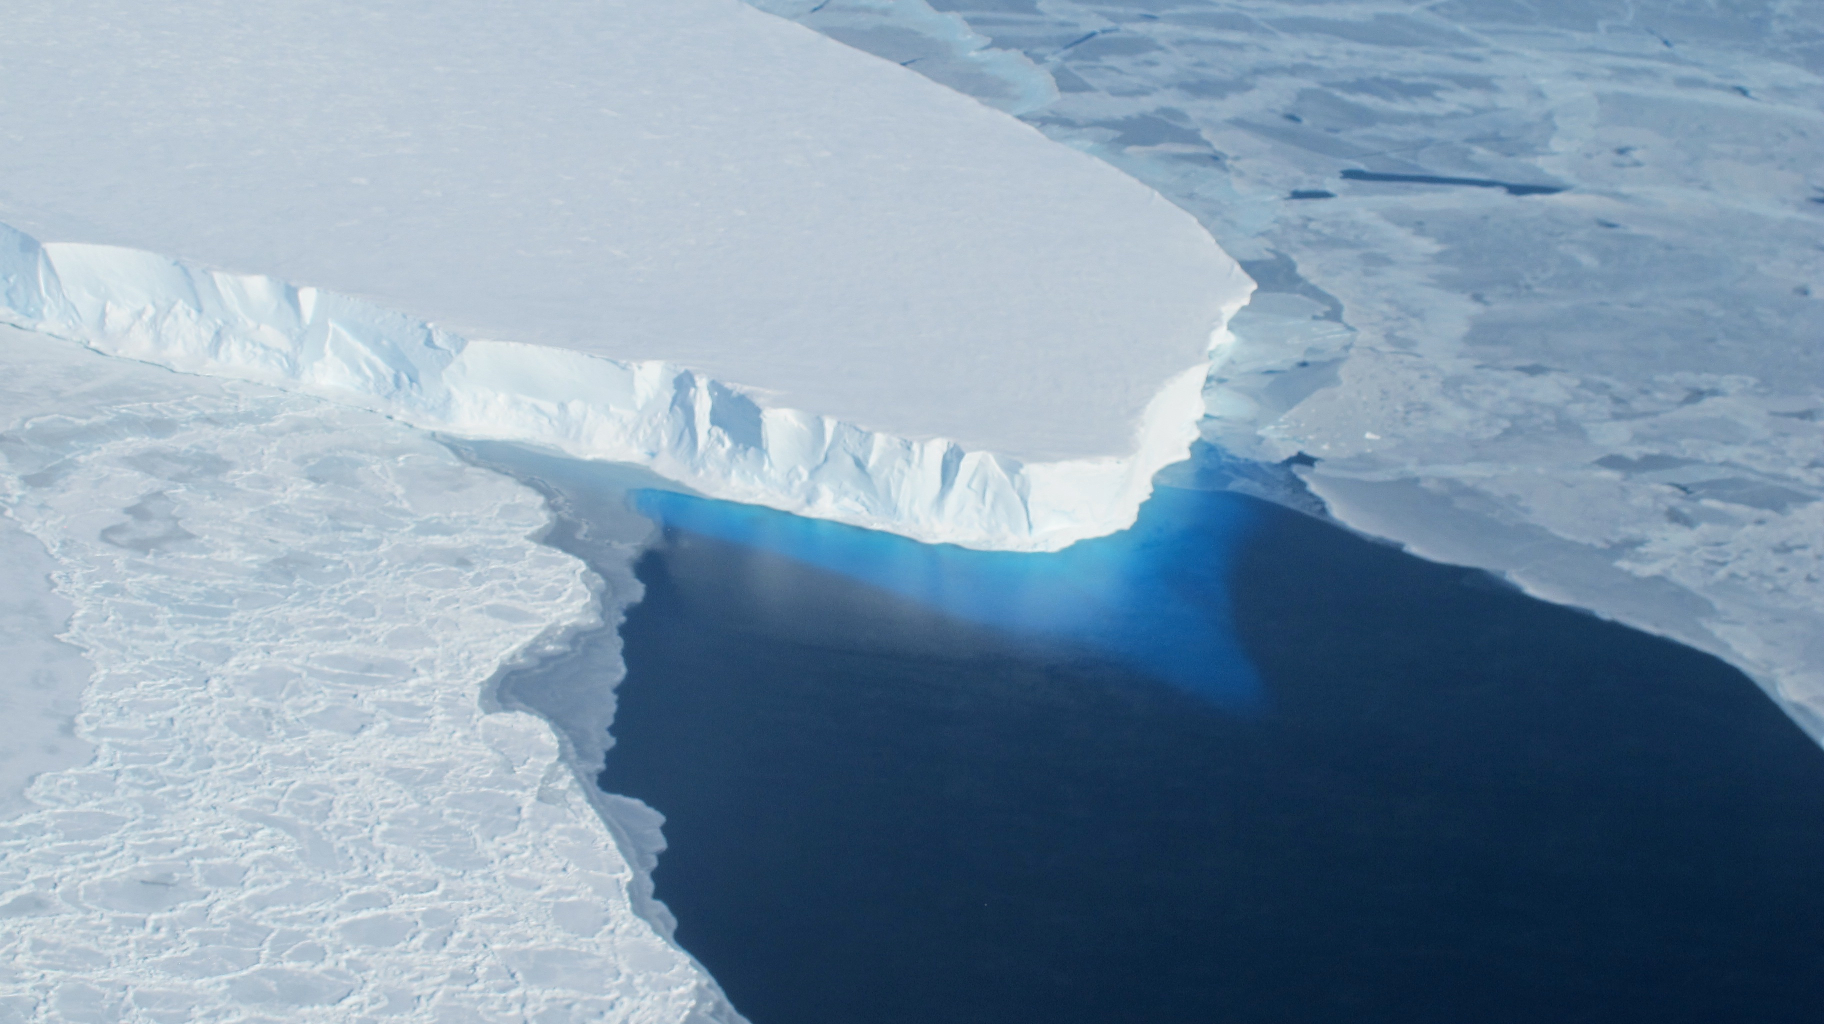
\includegraphics[width=1.0\textwidth]{supp4rignot-small}

\medskip
\tiny [ice shelf at Thwaites Glacier, Antarctic]
\end{center}
\end{frame}


\begin{frame}{models of ice shelves: they work}

\begin{itemize}
\item Ross ice shelf (Antarctica) velocity below
  \begin{itemize}
  \item[$\circ$] observed versus computed by SSA model in PISM
  \item[$\circ$] tuned: single, constant $A$
  \end{itemize}
\end{itemize}
\vspace{-0.3in}

\begin{center}
  \mbox{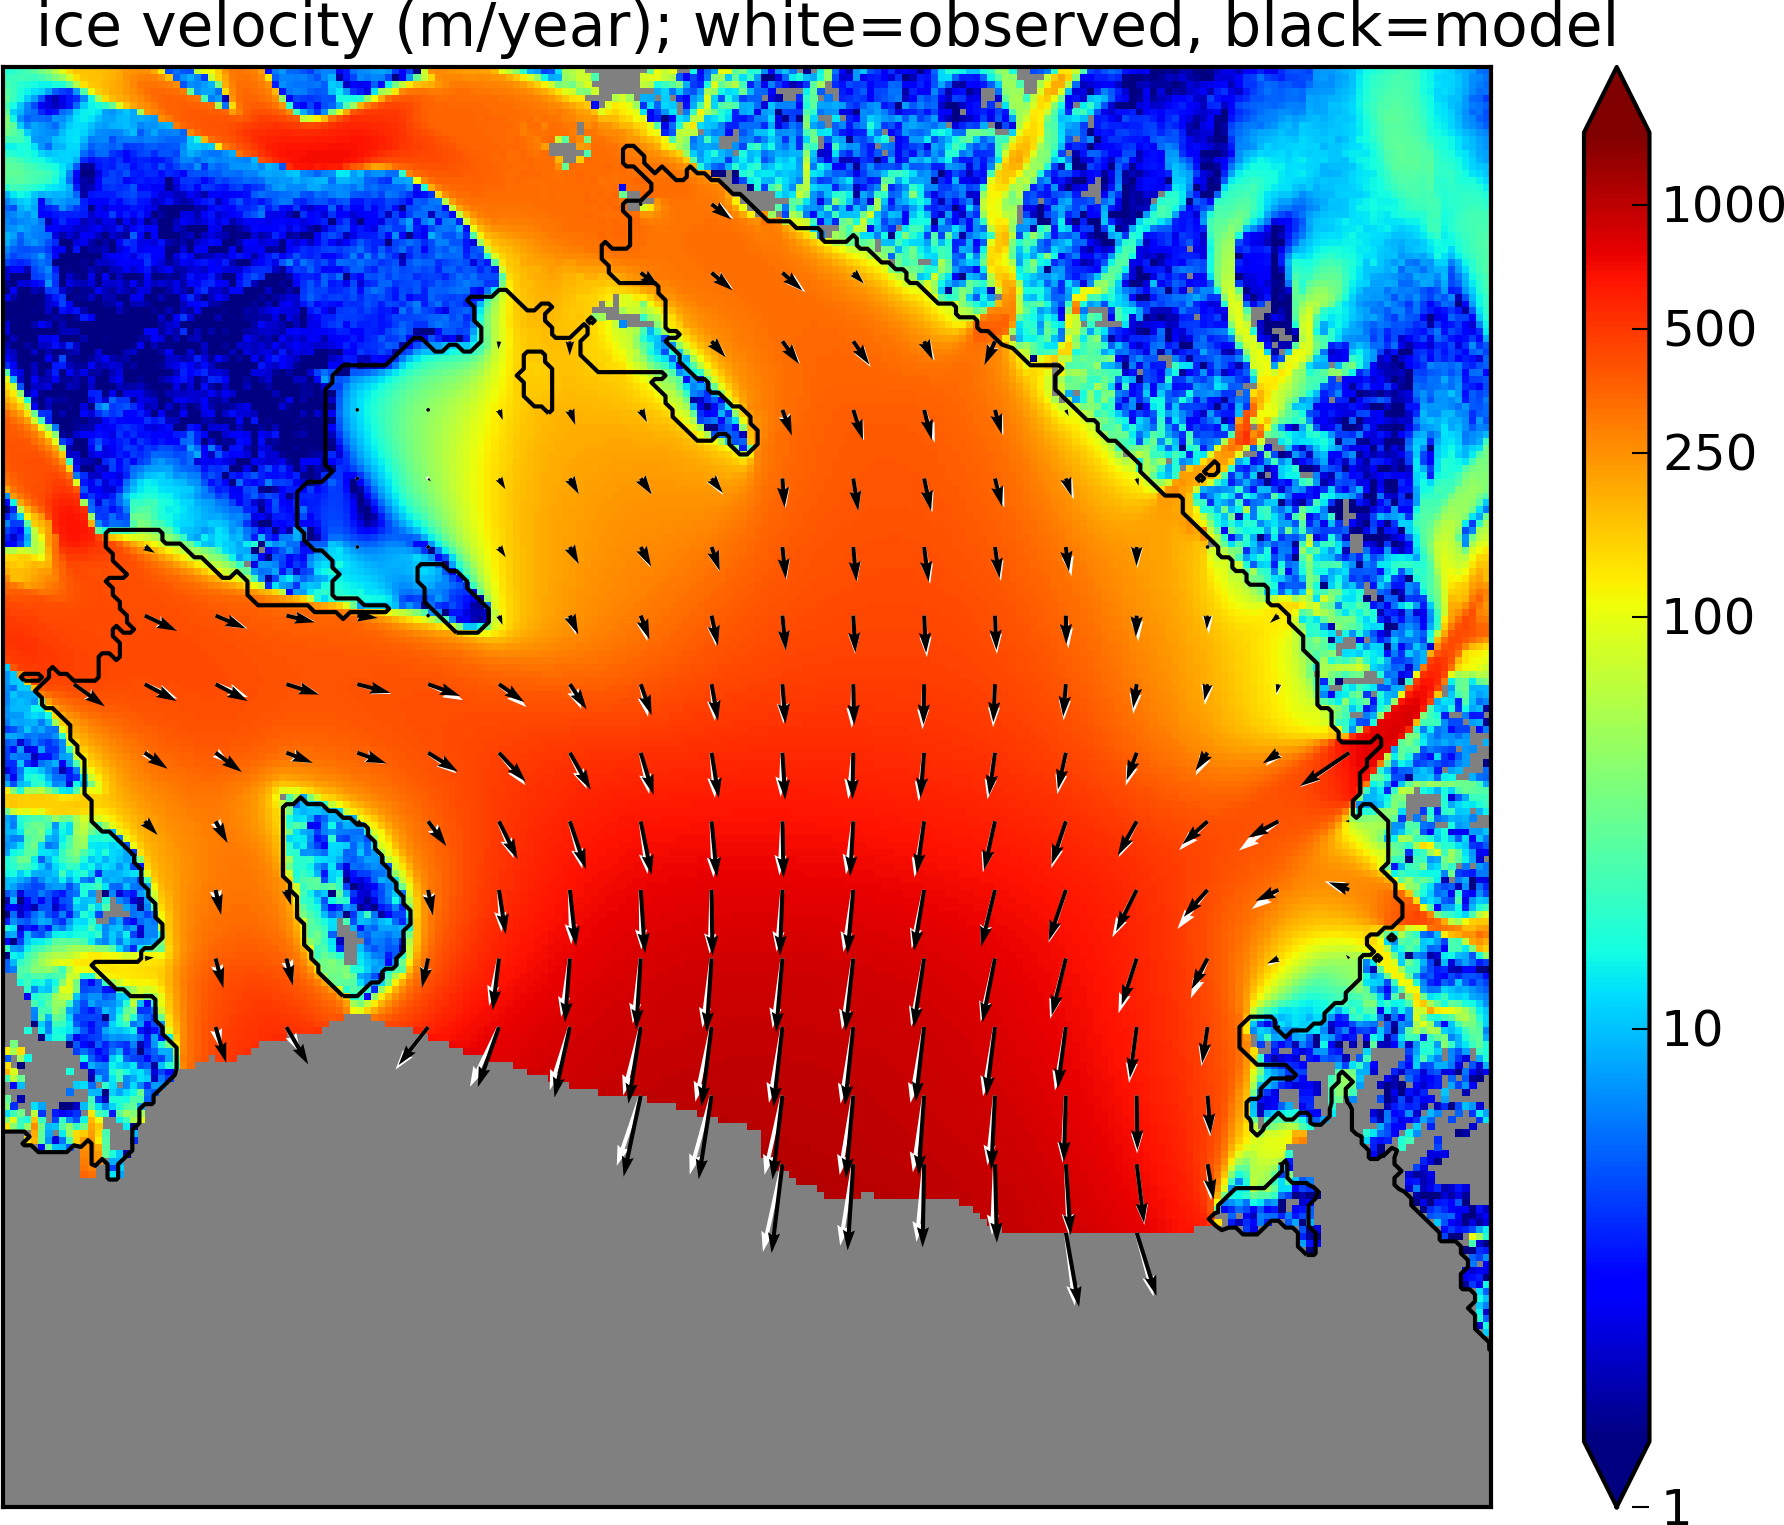
\includegraphics[width=0.58\textwidth]{rossquiver} \, 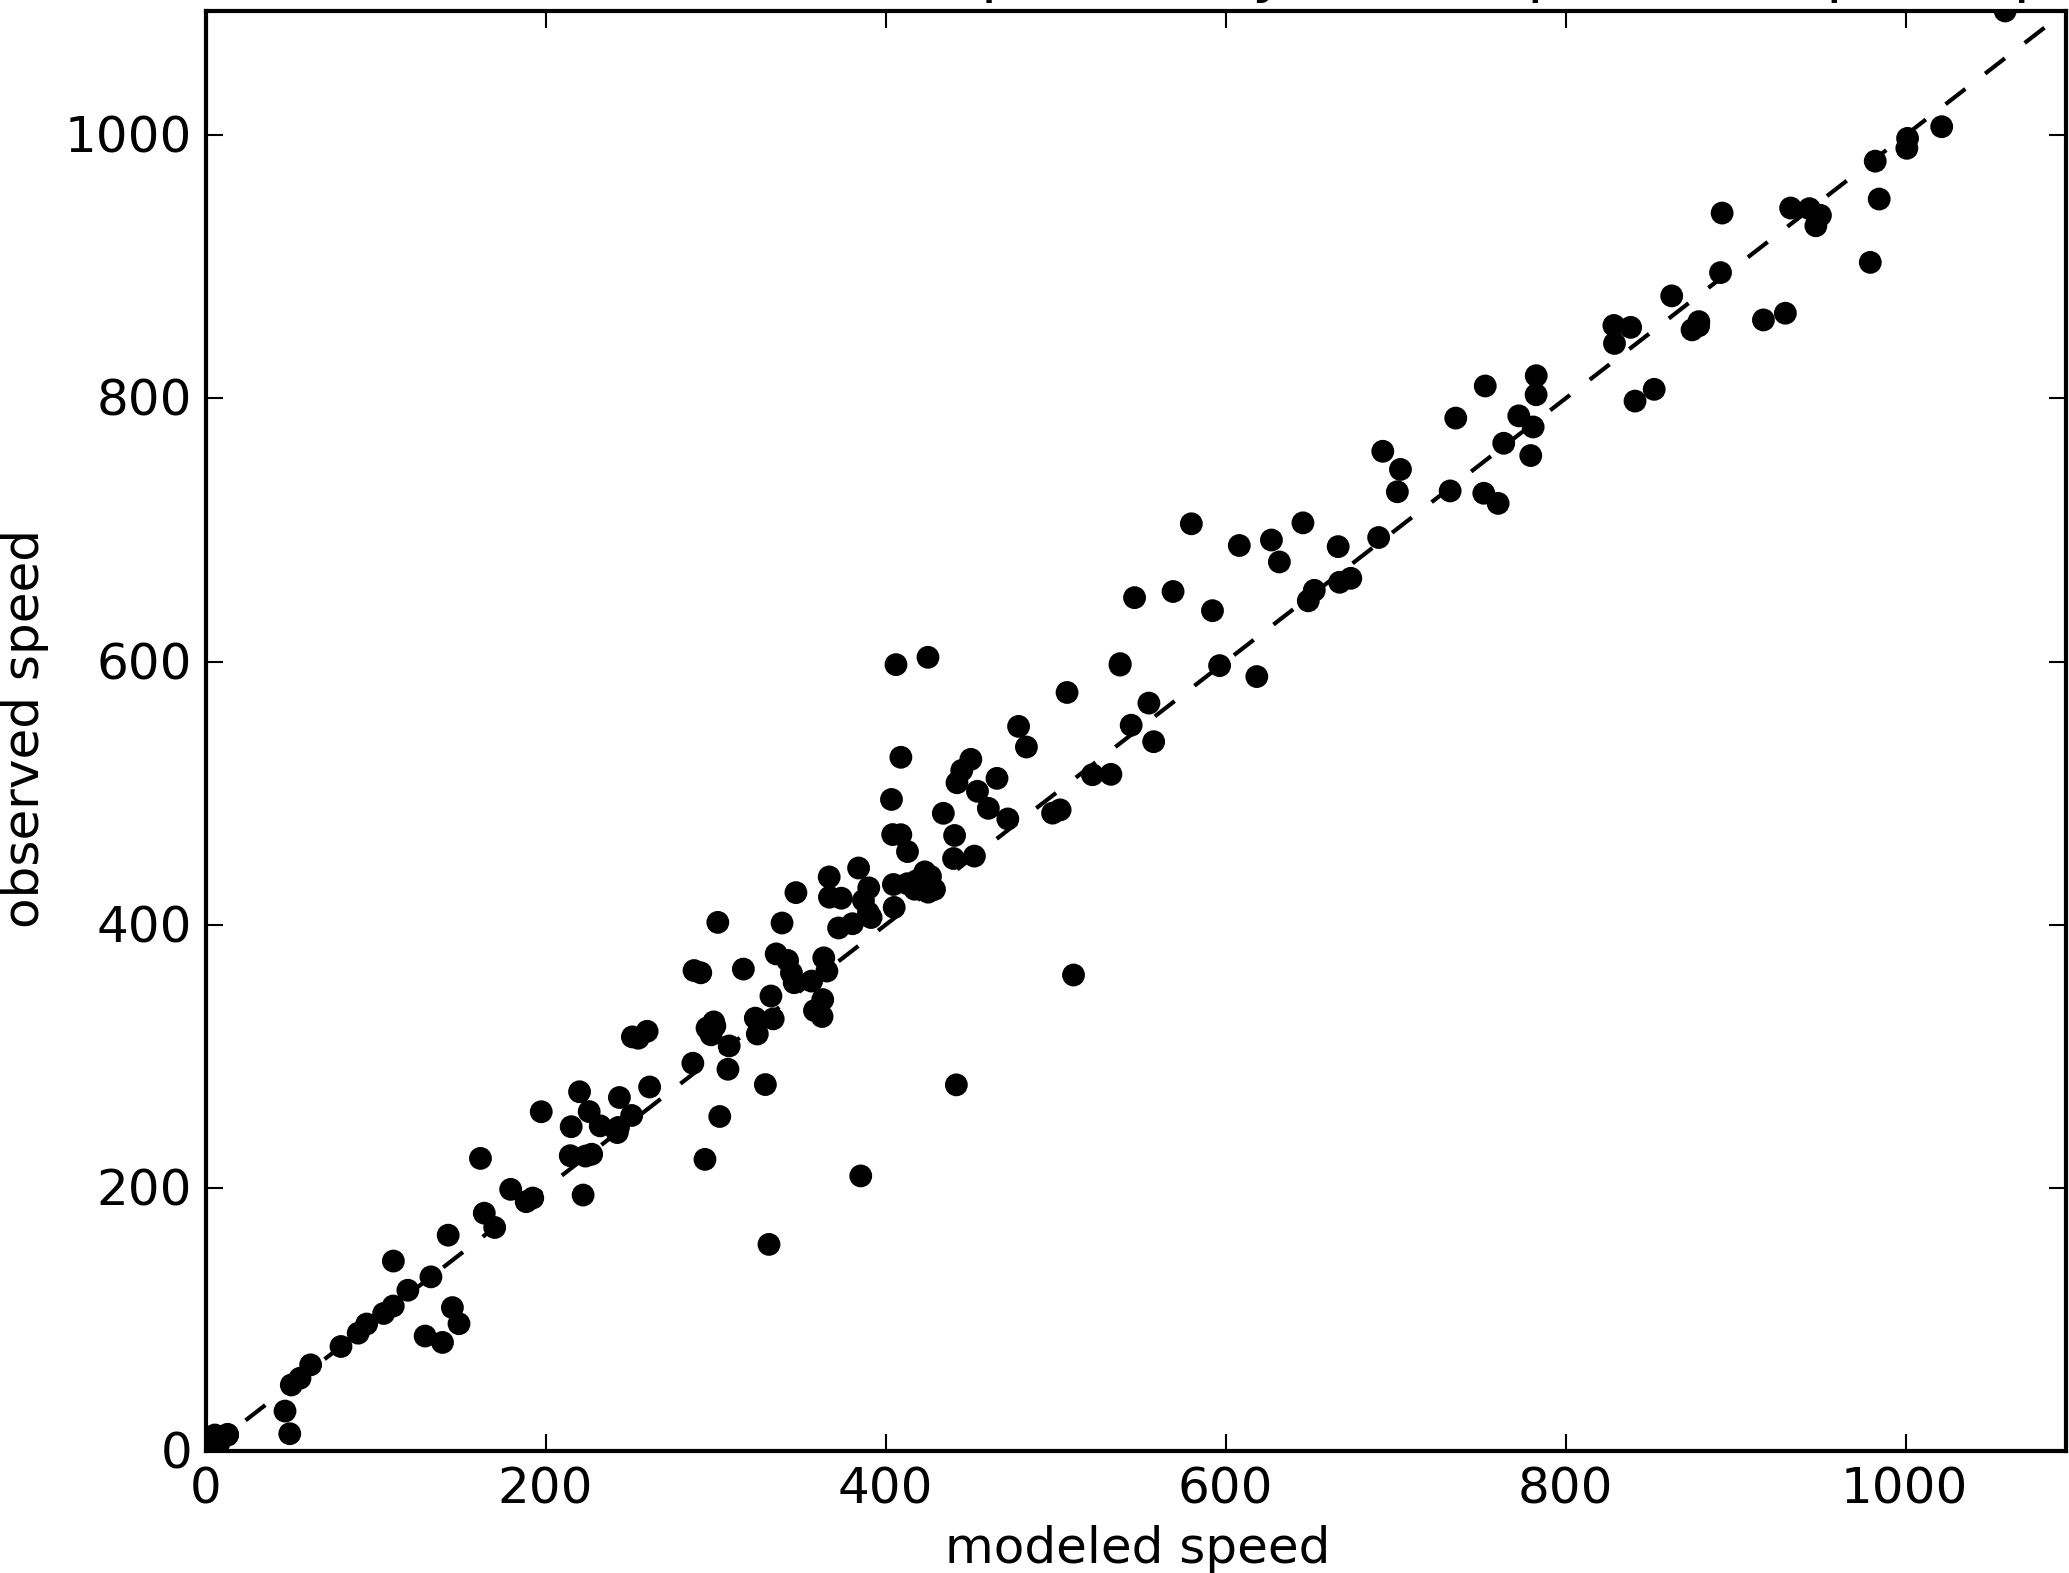
\includegraphics[width=0.48\textwidth]{rossscatter}}
\end{center}
\end{frame}


\begin{frame}
  \frametitle{ice streams: an analogy}

\begin{columns}
\begin{column}{0.6\textwidth}
\begin{itemize}
\item ice shelves have zero basal resistance
\item ice streams emerge where basal resistance is low enough
\item basal resistance is low if there is pressurized liquid water underneath the ice sheet
\item ice sheet is a membrane which connect sliding ice to upstream and/or lateral non-sliding ice
\end{itemize}
\end{column}
\begin{column}{0.4\textwidth}
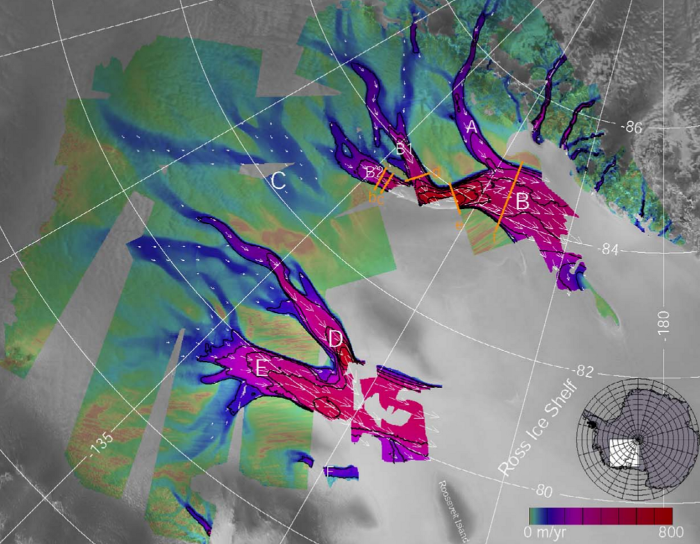
\includegraphics[width=\textwidth]{siple}

\vspace{0.3in}

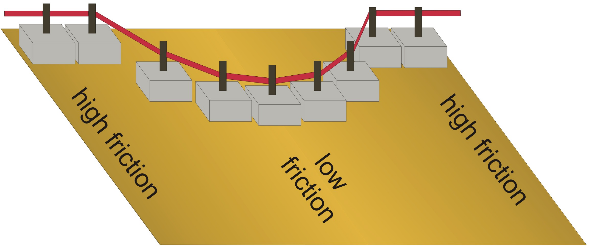
\includegraphics[width=1.1\textwidth]{schoof-sliders}
\end{column}
\end{columns}
\end{frame}


\section[on being right]{how do we know the numerical models are right?}

\begin{frame}
  \frametitle{moving grounding line in the lab}
  \framesubtitle{by Pegler et al.~(2014)}

\begin{center}

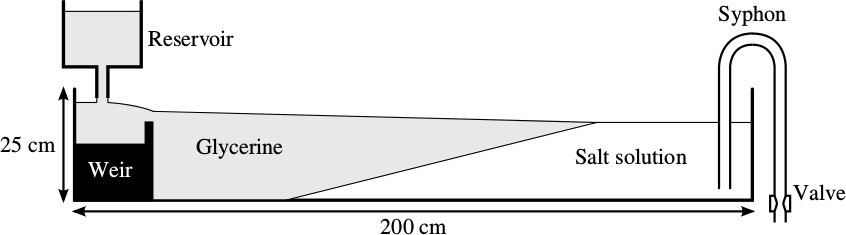
\includegraphics[width=0.7\textwidth]{pegler2014-grounding-line-schematic}

\vspace{1.0in}
[show movie]
\end{center}
\end{frame}


\begin{frame}{FIXME slide about exact solutions}
\end{frame}


\begin{frame}{FIXME slide about MMS}
\end{frame}


% SHOW Andy RCP runs



\section*{conclusion}

\begin{frame}
  \frametitle{conclusion}
  \framesubtitle{thanks for listening!}

\begin{center}
FIXME
\end{center}

\end{frame}


\end{document}
